\documentclass[11pt,english,a4paper]{memoir}
\usepackage[T1]{fontenc}
\usepackage[utf8]{inputenc}

\usepackage{textcomp}

\usepackage[opticals,textosf,mathlf,swash,minionint,amsbb]{MinionPro}
%\usepackage[osf]{mathpazo}
\usepackage[final]{microtype}
\usepackage{pifont}

\usepackage{babel}
\usepackage{color}

\usepackage[hidelinks,final,bookmarksopen=true]{hyperref}

\hypersetup {
  pdftitle = {CV of Dr. Heinrich Küttler},
  pdfauthor = {Heinrich Küttler}
}

\usepackage[absolute]{textpos}
\usepackage{graphicx}

\makeatletter

\settrimmedsize{297mm}{210mm}{*}
\setlength{\trimtop}{0pt}
\setlength{\trimedge}{\stockwidth}
\addtolength{\trimedge}{-\paperwidth}
\settypeblocksize{265mm}{157mm}{*}
\setulmargins{*}{*}{1}
\setlrmargins{*}{*}{1}
\setheadfoot{\onelineskip}{1.5\onelineskip}
\setheaderspaces{*}{\onelineskip}{*}
\checkandfixthelayout

\renewcommand{\footnoterule}{}
\setlength{\footmarkwidth}{-1.0em}
\setlength{\footmarksep}{-\footmarkwidth}
\footmarkstyle{#1~}
\renewcommand*{\@makefnmark}{\hbox{\textsuperscript{\@thefnmark}}}

\newcommand{\hairspace}{\kern .04167em}
\definecolor{Maroon}{cmyk}{0, 0.87, 0.68, 0.32}
\definecolor{halfgray}{gray}{0.55}
\definecolor{RoyalBlue}{cmyk}{1, 0.50, 0, 0}

\newcommand{\smallcaps}[1]{\textsc{\MakeLowercase{#1}}}

\copypagestyle{heinercv}{empty}
\makeoddfoot{heinercv}%
            {\color{halfgray}\footnotesize\smallcaps{CV of Heinrich
            Küttler, page \thepage\ of \thelastpage}}{}{}
\makeevenfoot{heinercv}%
             {\color{halfgray}\footnotesize\smallcaps{CV of Heinrich
             Küttler, page \thepage\ of \thelastpage}}{}{}
\pagestyle{heinercv}

\newcommand{\heinrichkuettleratgmaildotcom}{hein\rlap{\textcolor{white}{hugo@egon}}rich.kue\rlap{\textcolor{white}{@symmetry is overrated}}ttler@\rlap{\textcolor{white}{yesihatespamspamspam}}g\rlap{\textcolor{white}{spam@spam@spam!}}ma\rlap{\textcolor{white}{.de}}il.com}
\renewcommand{\heinrichkuettleratgmaildotcom}{hein\rlap{\textcolor{white}{ - }}rich.kue\rlap{\textcolor{white}{ }}ttler@\rlap{\textcolor{white}{}}g\rlap{\textcolor{white}{}}ma\rlap{\textcolor{white}{}}il.com}
\newcommand{\muelleratlmudotde}{mue\rlap{\textcolor{white}{hugo@egon}}ll\rlap{\textcolor{white}{@symmetry is overrated}}er@\rlap{\textcolor{white}{yesihatespamspamspam}}l\rlap{\textcolor{white}{spam@spam@spam!}}mu\rlap{\textcolor{white}{.com}}.de}
\newcommand{\heineratgoogledotcom}{hein\rlap{\textcolor{white}{hugo@egon}}e\rlap{\textcolor{white}{@symmetry is overrated}}r@\rlap{\textcolor{white}{yesihatespamspamspam}}g\rlap{\textcolor{white}{spam@spam@spam!}}oo\rlap{\textcolor{white}{.de}}gle.com}
\newcommand{\juergenvoigtattudresdende}{juer\rlap{\textcolor{white}{hugo@egon}}gen.voi\rlap{\textcolor{white}{@symmetry is overrated}}gt@\rlap{\textcolor{white}{yesihatespamspamspam}}tu-\rlap{\textcolor{white}{spam@spam@spam!}}dres\rlap{\textcolor{white}{.com}}den.de}

\newcommand{\red}{\color{Maroon}}

\newcommand{\header}[1]{%
  \addlinespace[2ex]
  & \large{\red\textsc{\MakeLowercase{#1}}} \tabularnewline
  \midrule}

\newcommand{\n}{\tabularnewline}
\newcommand{\bull}{\Pisymbol{MinionPro-Extra}{146}~~}
\newcommand{\nobull}{\phantom{\bull}}

\newcommand{\Cpp}{C\kern-.03em\raise.16ex\hbox{\small{+\kern-.03em+}}}

\makeatother

\begin{document}

\begin{textblock*}{3.7cm}(135mm,17mm)
  %  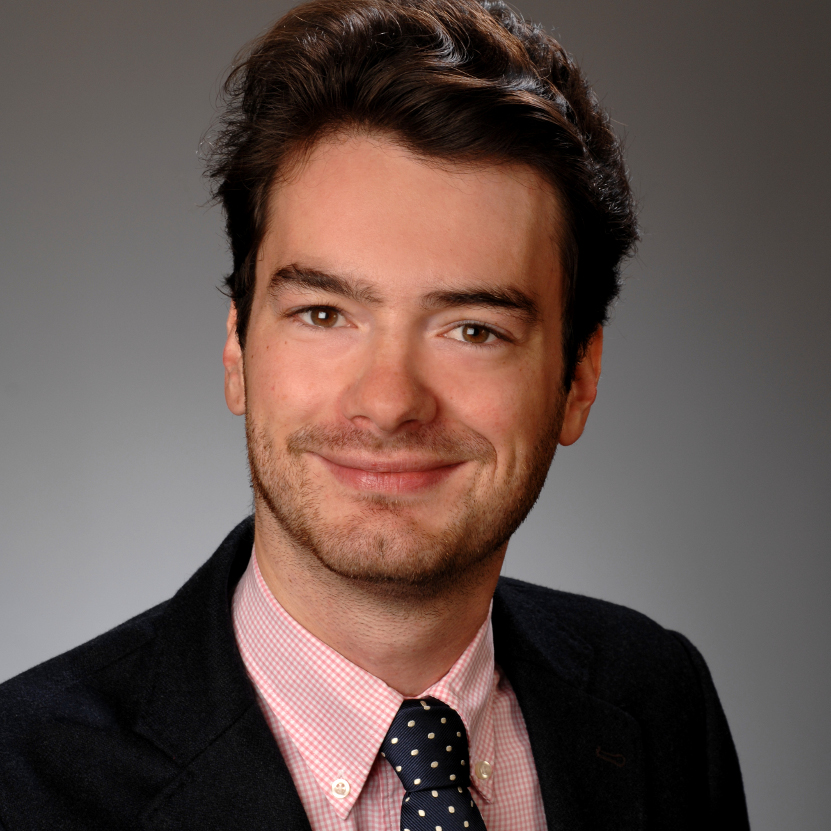
\includegraphics[width=3.7cm]{Foto_Heinrich_Kuettler_web.jpg}%
\begin{tabular}{rl}
  %% & \textbf{Dr. Heinrich Küttler} \n
  %% & Kreittmayrstr. 19 \n
  %% & 80335 München, Germany \n
  %% & \heinrichkuettleratgmaildotcom \n
  %% & +49 (0)163 2872\,914 \n \addlinespace
  & 27 Basterfield House \n
  & Golden Lane Estate \n
  & \smallcaps{EC1Y\,0TP} London, {UK} \n
\end{tabular}
\end{textblock*}

\begin{center}
%{\Large\textssc{lebenslauf von heinrich küttler} \par \bigskip}

%Danziger Straße 10 \textperiodcentered\ 85386 Eching \\
%\textit{hein\rlap{\textcolor{white}{hugo@egon}}rich.kue\rlap{\textcolor{white}{@symmetry is overrated}}ttler@\rlap{\textcolor{white}{yesihatespamspamspam}}go\rlap{\textcolor{white}{spam@spam@spam!}}oglema\rlap{\textcolor{white}{.de}}il.com}

%\bigskip

\begin{tabular}{rl}
  %% & \textbf{Dr. Heinrich Küttler} \n
  %% & Kreittmayrstr. 19 \n
  %% & 80335 München, Germany \n
  %% & \heinrichkuettleratgmaildotcom \n
  %% & +49 (0)163 2872\,914 \n \addlinespace
  & \textbf{CV of Heinrich Küttler} \n
  & \heineratgoogledotcom \n
  & +44 7760 998789 \n \addlinespace
  & Born 13 December 1985 in Zwickau, Germany \n \addlinespace[0.5ex]

  \header{Education}
  March 2010        & \textbf{LMU München, Germany} \n
  -- September 2014 & PhD in Mathematical Physics \n
  & \bull Cumulative grade 0.9, \textit{magna cum laude} \\
  & \nobull (Dissertation: 1.0, \textit{magna cum laude}, Disputation:
  0.7, \textit{summa cum laude}) \n
  & \bull Four publications in highly-respected journals, among others in \\
  & \nobull Communications in Mathematical Physics

  \n \addlinespace
  October 2004  & \textbf{TU Dresden, Germany} \n
  -- July 2009  & Major: Mathematics, \ Minor: Physics and Computer Science \n
  & \bull Diploma grade 1.0, with distinction \n
  & \bull Diploma exam included: PDEs, Variational Calculus,\\
  & \nobull Probability Theory, Java, Security and Cryptography

  %\n \addlinespace
  %July 2004 & \textbf{Peter-Breuer-Gymnasium, Zwickau, Germany} \n
  %& \bull German Abitur, cumulative grade 1.4

  \n
  \header{Scholarships}
  February 2007 & \textbf{German National Academic Foundation (Studienstiftung)} \n
  & Stipend awarded by Germany's largest and oldest sponsorship organisation
  \n
  & \bull Nomination based on undergraduate results (top 2\% of class
  eligible for \\
  & \nobull two-day assessment centre) \n
  & \bull Took part in regular meetings, attended summer school

  \n
  \header{Work Experience}
  July 2015 & \textbf{Google UK, Ltd., London} \n
  -- present & Technical Solutions Consultant, gTech \n
  & \bull Provide consulting services to Google's publishing partners
  and develop \\
  & \nobull cutting-edge solutions as the technical lead \n
  & \bull Analyse large amounts of customer and internal data to
  identify trends \\
  & \nobull and provide strategic insights

  \n \addlinespace
  March 2010 & \textbf{LMU München, Germany} \n
  -- January 2015 & Research Assistant at the \href{http://www.mathematik.uni-muenchen.de/forschung/arbeitsgruppen/analysis/index.html}{Mathematics Institute} \n
  & \bull Organisation of University classes, teaching in several
  subjects
  %(among \\
  %& \nobull them mathematical analysis, functional analysis, and
  %complex analysis)
  (see \\
  & \nobull \href{http://www.math.lmu.de/~kuettler}{www.math.lmu.de/\textasciitilde{}kuettler}
  for full list)
  \\
  & \bull
  Design and management of written and oral exams \n
  & \bull Various talks and scientific presentations in seminars and
  conferences

  \n \addlinespace
  August 2009      & \textbf{TU München, Germany} \n
  -- February 2010 & Research Assistant at the \href{http://www.lnm.mw.tum.de/}{Institute for Computational Mechanics} \n
  & \bull Management of the IT infrastructure, including the \\
  & \nobull high-performance cluster and workspaces for $> 30$ researchers \\
  & \bull Development of finite element code in \Cpp\ for biofluid \\
  & \nobull mechanics applications, e.g., airflow in lung respiration

  \n
  \header{Internship}
  July 2008       & \textbf{University of Leicester, UK} \n
  -- August 2008  & Intern at the \href{http://www.le.ac.uk/biology/phh4/}{Department of Biology} \n
  & \bull Creation of software to analyse repetitive motifs in
  \textit{Drosophila} \\
  & \nobull DNA sequences to help find their evolutionary descent \n
  & \bull Co-authored a publication about the results, published in \\
  & \nobull Molecular Biology and Evolution, Oxford University Press
\end{tabular}

\begin{tabular}{rl}
  \header{Skills}
  Languages & \bull German: native, \ English: fluent \n \addlinespace

  Computer Skills & \bull Coding experience in Python, Ruby, Java, \Cpp, \\
                  & \nobull released on Google Play App Store and other platforms \n
                  & \bull MS Office, \TeX\ literacy
  %\n \addlinespace
  \n
  \header{Other interests}
  %% Politics        & \bull Member of European Students for Liberty, \n
  %% & \nobull participant in international meetings and conferences  \n \addlinespace

  %% Community       & \bull Volunteer work for the local church, e.g.,
  %%                   arranging accommodation \\
  %%                 & \nobull for foreign visitors of \textit{Ökumenischer Kirchentag} \n \addlinespace
  & \bull Various Open Source projects
  (see \href{https://github.com/heiner}{github.com/heiner}) \n
  & \bull Amateur guitarist, typography enthusiast,
  hobby economist,  \\
  & \nobull and Bob Dylan aficionado \n
  & \bull Member of DANTE society \n \addlinespace
  9--22 September 2007
  & \bull Attended summer school of Studienstiftung in Olang, South Tyrol, \\
  & \nobull part of the Friedrich Schiller study/acting team

  \n
  \header{Publications}
  PhD thesis & \textit{Anderson's Orthogonality Catastrophe} \\
  & \href{http://edoc.ub.uni-muenchen.de/17442/}{LMU München, 2014} \n \addlinespace

  Mathematical Articles
  & \textit{The Exponent in the Orthogonality Catastrophe for Fermi Gases} \\
  & Martin Gebert, Heinrich Küttler, Peter Müller, Peter Otte \\
  & \href{http://arxiv.org/abs/1407.2512}{arXiv:1407.2512}, to appear
  in J. Spectr. Theory \n \addlinespace

  & \textit{Anderson's Orthogonality Catastrophe} \\
  & Martin Gebert, Heinrich Küttler, Peter Müller \\
  & \href{http://dx.doi.org/10.1007/s00220-014-1914-3}{Comm. Math. Phys. 329 (3), pages 979--998,
  Springer, 2014} \n \addlinespace

  & \textit{Anderson's Orthogonality Catastrophe for One-Dimensional Systems}
  \\
  & Heinrich Küttler, Peter Otte, Wolfgang Spitzer \\
  & \href{http://dx.doi.org/10.1007/s00023-013-0287-z}{Ann. Henri Poincaré \,15 (9), pages 1655--1696, Springer, 2014}

  \n \addlinespace
  Other peer-reviewed & \textit{The Repetitive DNA of Drosophila:
  Concerted Evolution at Different}
  \\
  articles & \textit{Genomic Scales and Association with Genes} \\
  & Gustavo C. S. Kuhn, Heinrich Küttler, Orlando Moreira-Filho, \\
  & John S. Heslop-Harrison \\
  & \href{http://dx.doi.org/10.1093/molbev/msr173}{Mol. Biol. Evol. 29 (1), pages 7--11, Oxford University Press, 2012}

  %% \n
  %% \header{Reference}
  %% PhD advisor & \textbf{Dr. Peter Müller}, Professor at Mathematics Institute, LMU München
  %% \\
  %% & Tel: +49 (0)89 2180\,4434, \ Email: \muelleratlmudotde

  %% \n \addlinespace

  %% Supervisor         & \textbf{Dr. Jürgen Voigt}, Professor at Department of
  %% Mathematics, TU Dresden \\
  %% for diploma thesis &
  %% Tel: +49 (0)351 463\,33790, \ Email: \juergenvoigtattudresdende
\end{tabular}

\end{center}

% In Deutschland: CV unterschreiben

%% \iftrue
%% %\iffalse
%%   \bigskip

%%   \hfill
%%   \includegraphics{signature}  \hspace*{-3.0em} \\
%%   \hspace*{\fill} Dr. Heinrich Küttler
%% \fi

\end{document}
